\documentclass[mathserif,9pt]{beamer}
\usepackage[T1]{fontenc}
\usepackage[utf8]{inputenc}
\usepackage[ngerman]{babel}        % German style for date, sections ...

%\usepackage{helvet}

% Teilweise nützeliche Pakete:
%\usepackage[USenglish,english,ngerman]{babel}
%\usepackage{fancyhdr}
%\usepackage{hyperref}
%\usepackage{graphicx}
%\usepackage{array}
%\usepackage{tikz}
%\usepackage{fancyvrb}
%\usepackage{ctable}
%\usepackage{longtable}
%\usepackage{hhline}
%\usepackage{varioref}
%\usepackage{wrapfig}
%\usepackage{subfigure}
%\usepackage{eurosym}
%\usepackage{hvfloat}
%\usepackage{tabularx}
%\usepackage{bibgerm}
%\usepackage{listings}
%\usepackage{color}

\usepackage{fbtechnik-slides-100917}
\usepackage{graphicx}    % custom beamer style file: HS Emden/Leer

\title[Einarmiger Arduit]{Einarmiger Arduit}
\subtitle{Glücksspiel kann Süchtig machen}
\author{Arbeitstechniken Gruppe 64}
\institute{Franziska Massmann \; Jonas Nikolić \; Lukas Pensler \; Simon Struck}
\date{\today}

%\date[31. August 2010]{\vspace{-30pt}\\31. August 2010\\[10pt]
%{\scriptsize
%\begin{tabular}{ll}
%	Erstprüfer:	& Prof. Dr. ... \\
%	Zweitprüfer:& Prof. Dr. ... \\
%\end{tabular}\\[-0cm]}}

\begin{document}
    \titleframe        % custom title frame with background logo

    \begin{frame}{Inhalt}
        %\begin{eblock}
        %\vspace{-1em}
        \tableofcontents
        %[hideallsubsections]
        %\end{eblock}
    \end{frame}

    \section{Wortschöpfung}
    \begin{frame}{}
        %			\framesubtitle{NANANA}
        \begin{block}{}
            \centering
            \Huge{
            Einarmiger Bandit \\
            + \\
            Arduino \\
            = \\
            Einarmiger Arduit}
        \end{block}
    \end{frame}

    \section{Unser Ziel}
    \begin{frame}{Unser Ziel}
        \begin{block}{Einarmiger Bandit mit einem Arduino und 7-Segment Displays}
            \begin{itemize}
                \item Spielekonsole nicht umsetzbar (zu teuer)
                \item Echte Rollen zu teuer und zu komplex
                \item LCD\,--\,Bildschirm nicht interessant genug
            \end{itemize}
        \end{block}
    \end{frame}

    \section{Umsetzung}

    \subsection{Schaltung}
    \begin{frame}{Schaltung}
        \begin{block}{Schaltung}
            \begin{minipage}[c]{0.6\textwidth}
                \begin{itemize}
                    \item Schieberegister aneinander gereiht für genug I/O
                    \item LEDs und 7-Segment-Displays simulieren Rollen
                \end{itemize}
            \end{minipage}
            \hfill
            \begin{minipage}[c]{0.3\textwidth}
                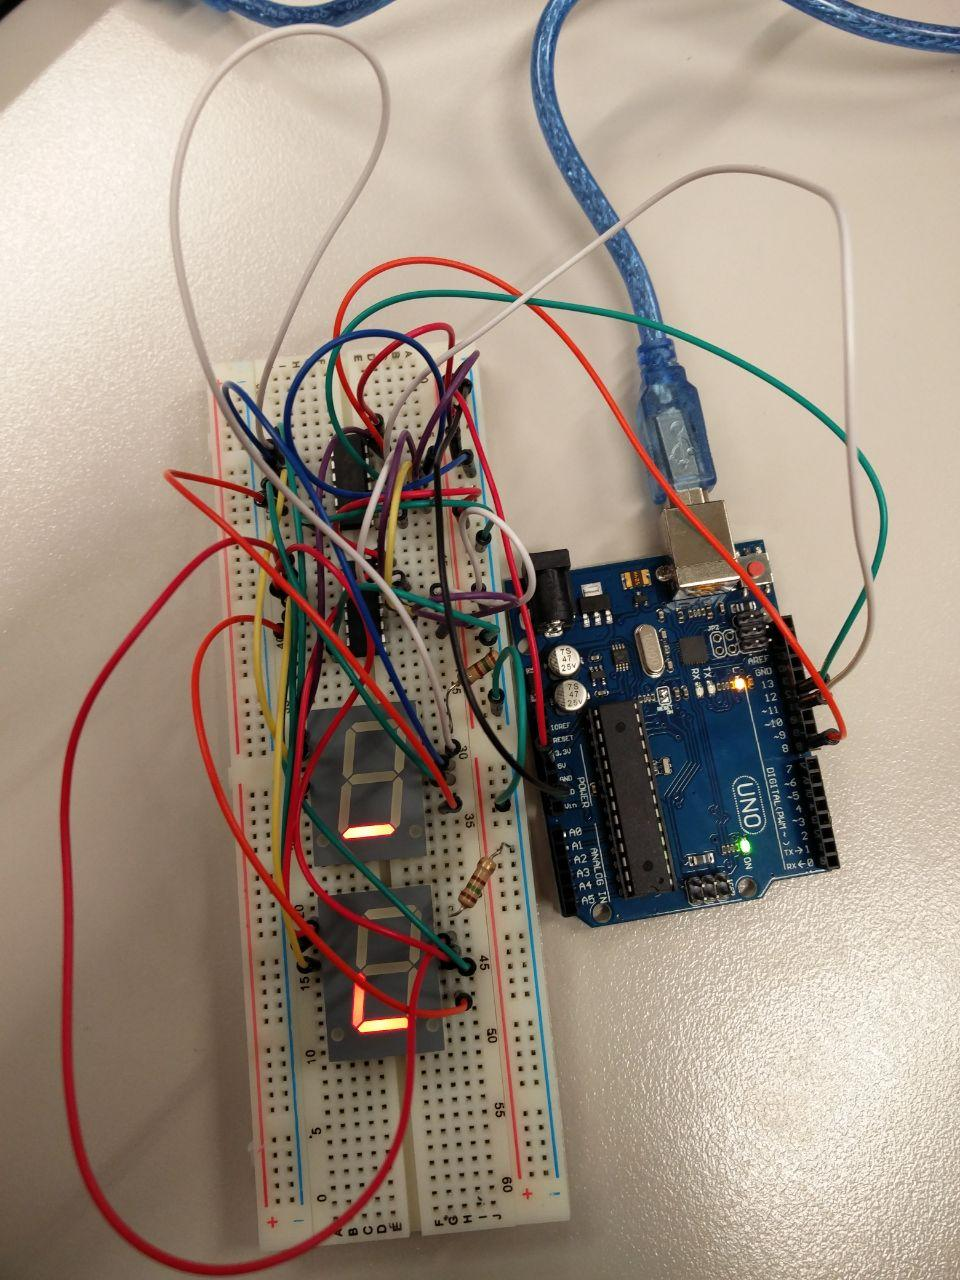
\includegraphics[width=\textwidth]{img/breadboard.jpg}
            \end{minipage}
        \end{block}
    \end{frame}

    \subsection{Code}
    \begin{frame}{Code}
        \begin{block}{Code}
            \begin{itemize}
                \item State Machine --- Kontrolliert animationen
                \item Interrupt --- Verarbeitet Input nur wenn welcher da ist
                \item Animationen --- Durch Algorithmus generiert um Platz zu sparen
            \end{itemize}
        \end{block}
    \end{frame}

    \subsection{Gehäuse}
    \begin{frame}{Gehäuse}
        \begin{block}{Gehäuse}
            \begin{itemize}
                \item Stabiles und leichtes Material
                \item Ergonomischer Bau
                \item Auf dem Tisch platziert sollen Rollen auf Augenhöhe sein
            \end{itemize}
            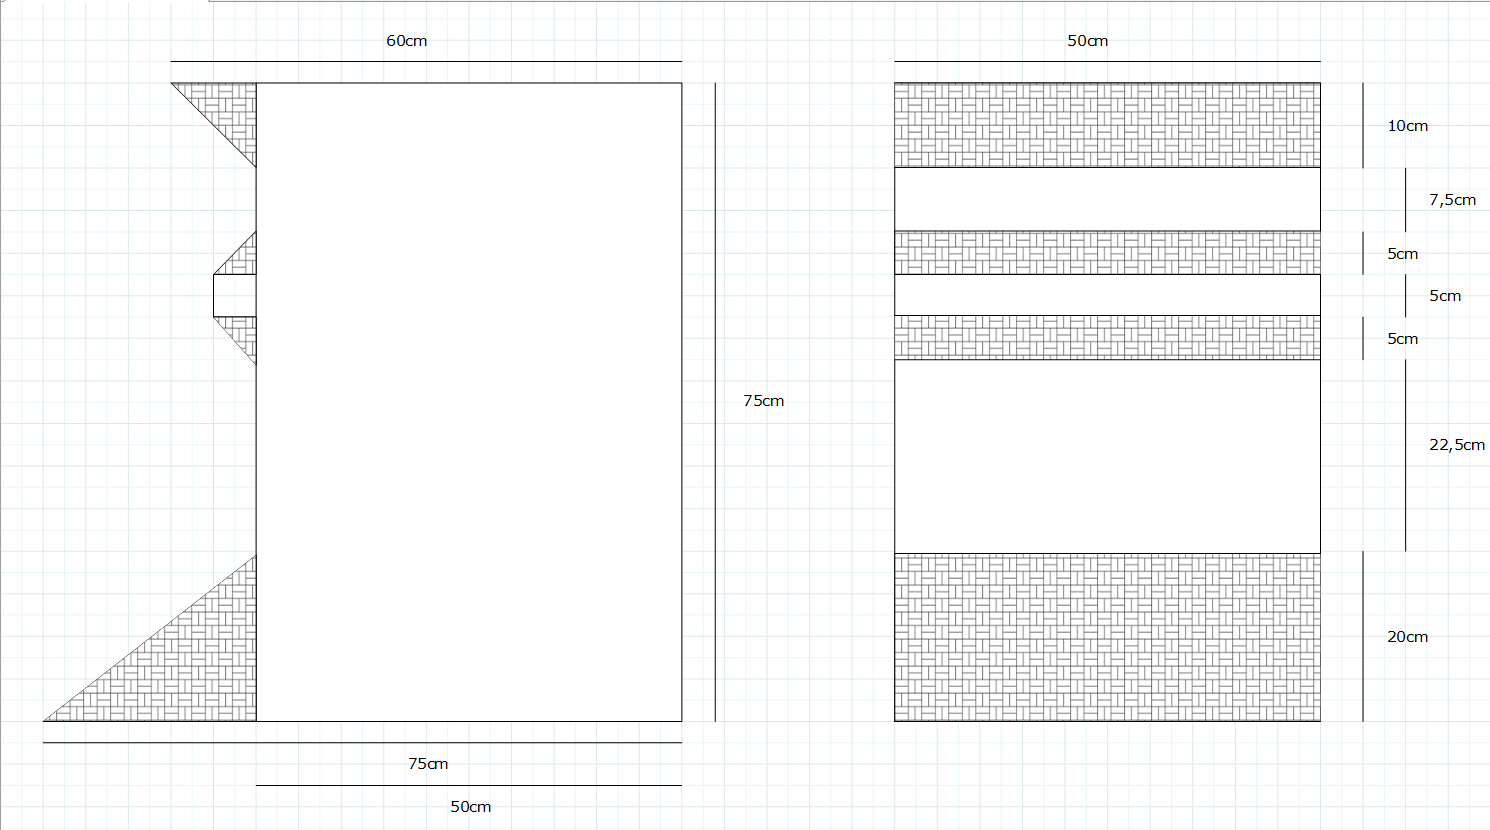
\includegraphics[height=0.4\paperheight]{img/gehause.png}
        \end{block}
    \end{frame}

    \subsection{Software}
    \begin{frame}{Software}
        \begin{block}{Software}
            \begin{itemize}
                \item Draw.io -- Diagramme erstellen
                \item Fritzing -- Schaltung Design
                \item Github -- Quellcode teilen
                \item Google Drive -- Dokumente teilen
                \item PlatformIO (Atom) -- Quellcode editieren
                \item Trello -- Organisieren
            \end{itemize}
        \end{block}
    \end{frame}
    \section{Demo}
    \begin{frame}
        \begin{block}{}
            \centering
            {\fontsize{100}{120}\selectfont Demo}
        \end{block}
    \end{frame}

    \section{Fazit}
    \begin{frame}
        \begin{block}{Fazit}
            \begin{block}{Aktueller Fortschritt:}
                \begin{itemize}{}
                    \item Code: In Arbeit
                    \item Gehäuse: Geplant
                    \item Schaltung: Prototyp im Bau
                \end{itemize}
            \end{block}
        \end{block}
    \end{frame}

    \section*{}
    \begin{frame}{Ende}
        \begin{block}{Ende}
            Vielen Dank für Ihre Aufmerksamkeit \ldots
        \end{block}
    \end{frame}

    %\begin{frame}{Literatur}
    %	\footnotesize
    %	\nocite*
    %	\bibliography{literatur}
    %	\bibliographystyle{geralpha}
    %\end{frame}

\end{document}
